% !TeX root = main.tex
% Slide della presentazione: da inserire nel documento Beamer esistente.

\begin{frame}{Outline}
  \tableofcontents
\end{frame}

\section{Introduction}

\begin{frame}{The Problem}
  \begin{columns}[c,onlytextwidth]
    \begin{column}{0.55\textwidth}
      \small
      \begin{itemize}
        \item \textbf{Mechanistic interpretability}
        aims to explain how neural networks produce predictions by identifying
        interpretable internal components and their causal relationships.

        \vspace{0.25cm}

        \item \textbf{Polysemanticity}
        occurs when a neuron activates in semantically unrelated contexts,
        making its behavior difficult to interpret.

        \vspace{0.25cm}

        \item \textbf{Superposition}
        is the hypothesis that networks represent more features than
        dimensions by using non-orthogonal directions.

        \vspace{0.25cm}

        \item \textbf{Sparsity}
        means that only a small subset of features is active for each input,
        limiting interference between features.
      \end{itemize}
    \end{column}

    \begin{column}{0.43\textwidth}
      \centering
      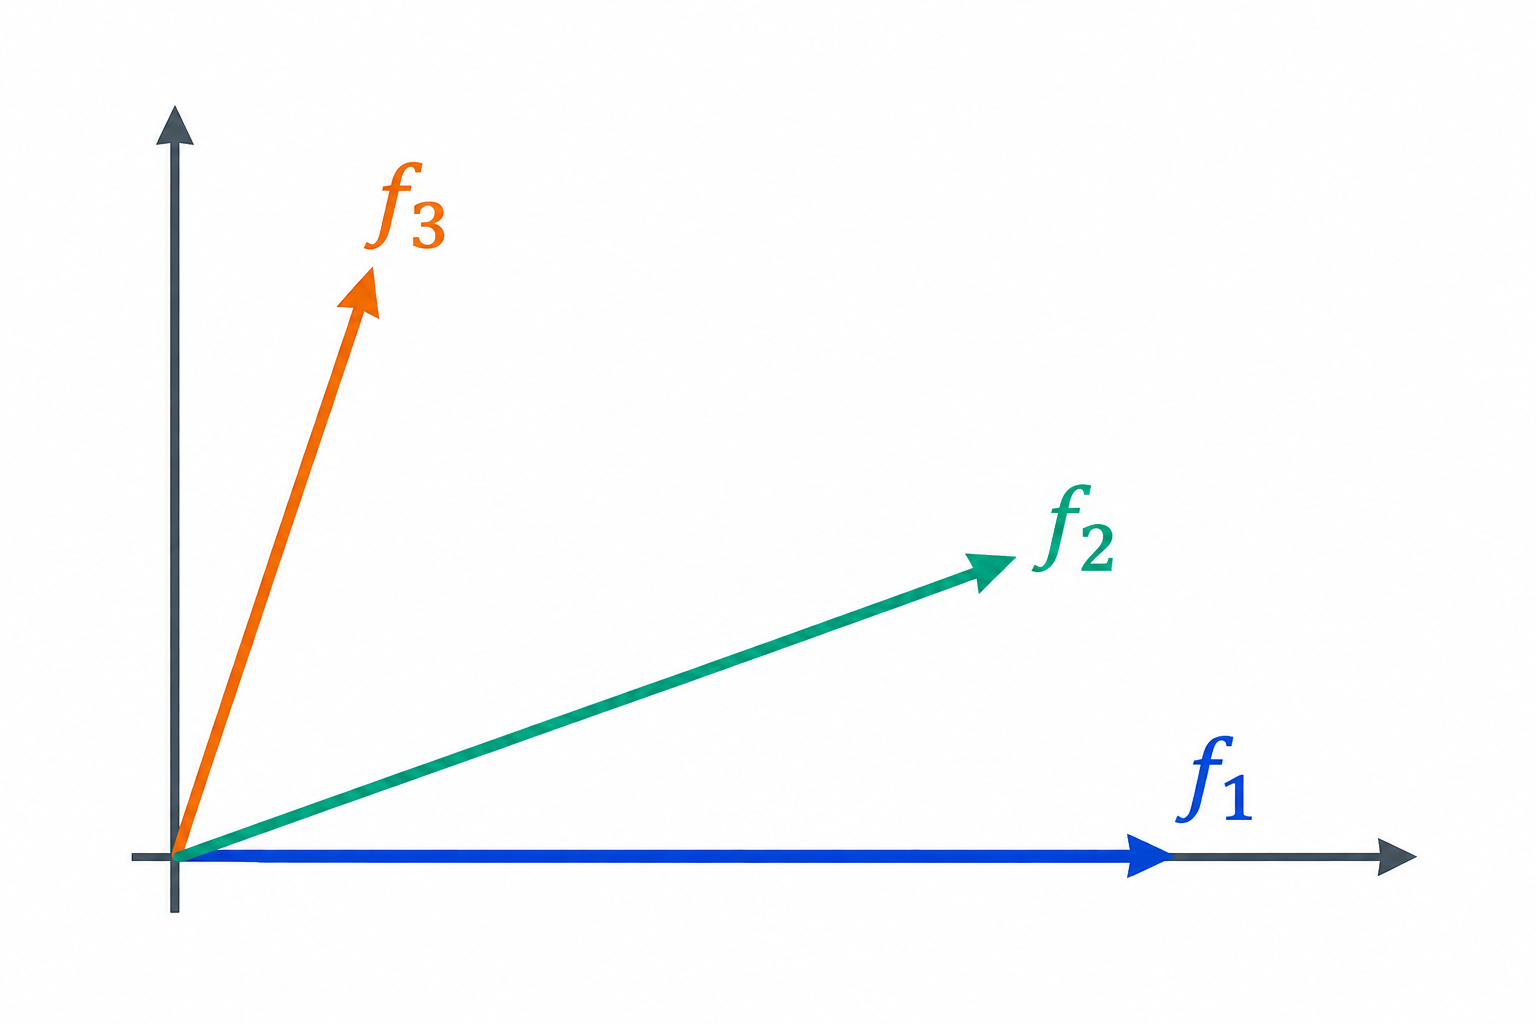
\includegraphics[width=\linewidth]{superposition.png}

      \vspace{0.3cm}

      $x = a_1 f_1 + a_2 f_2 + a_3 f_3$

      \vspace{0.2cm}

      {\footnotesize
        $f_i$: feature direction

        $a_i$: feature activation
      }
    \end{column}
  \end{columns}
\end{frame}

\begin{frame}[t]{Proposed Approach}
  \begin{center}
    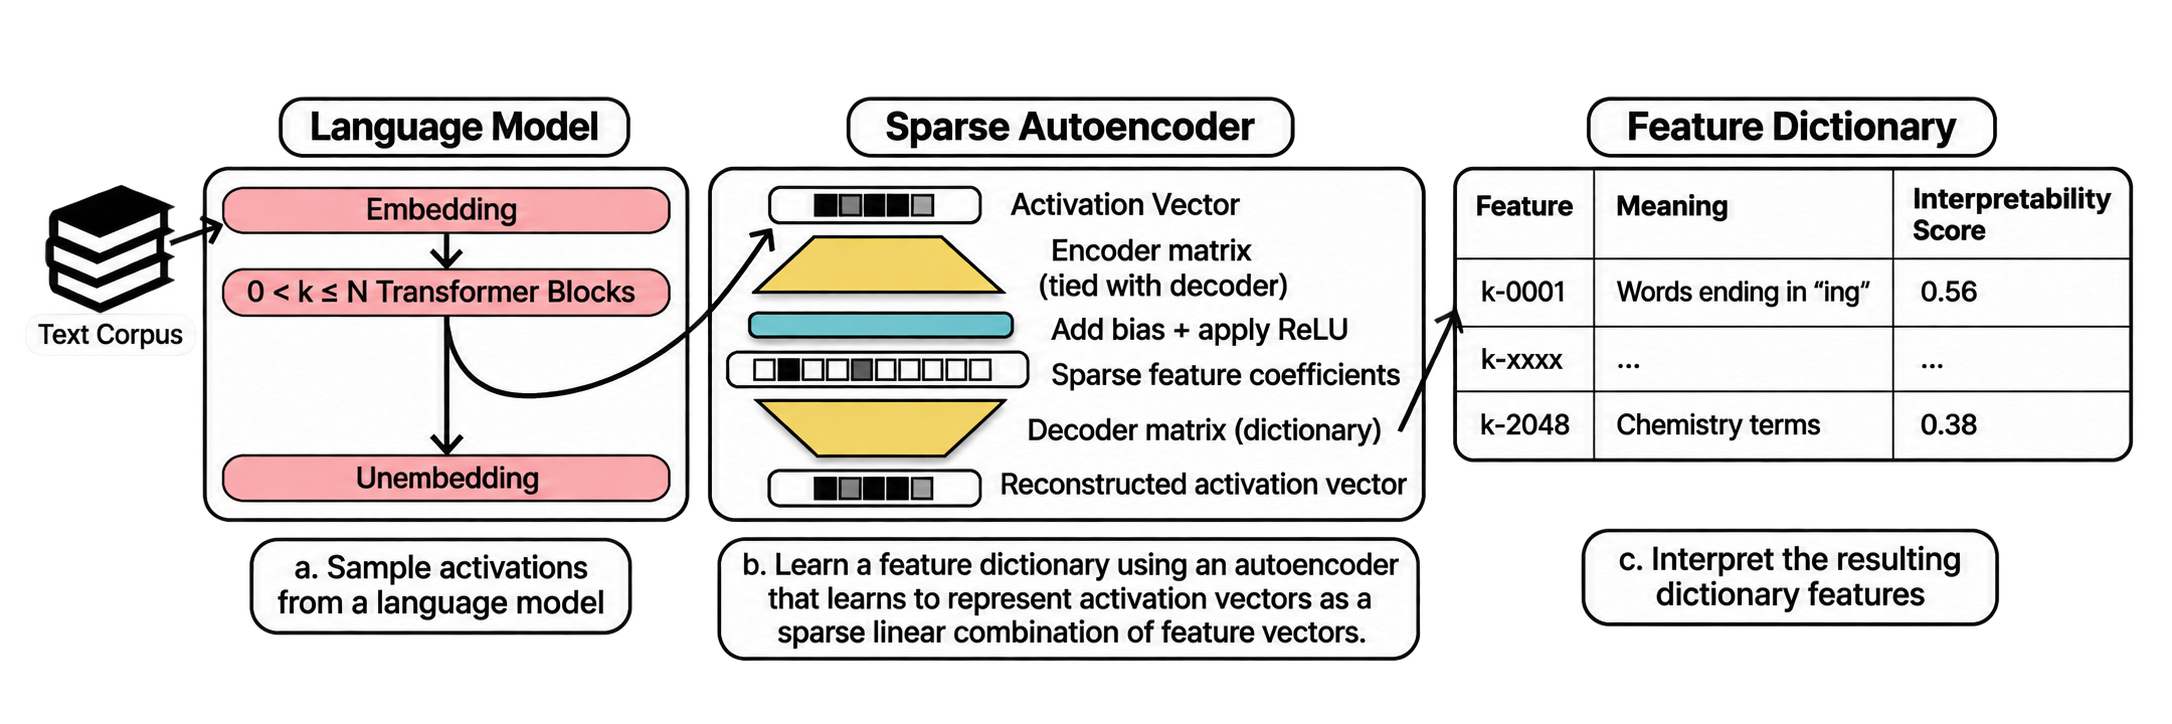
\includegraphics[
      width=0.95\textwidth,
      height=0.45\textheight,
      keepaspectratio
    ]{approach.png}
  \end{center}

  \medskip

  \begin{itemize}
    \item \textbf{Goal:} Recover meaningful feature directions so that
    activation vectors can be reconstructed as sparse linear combinations
    of these directions.

    \medskip

    \item \textbf{Method:} Train a Sparse Autoencoder on the internal
    activations of a pretrained language model.

    \medskip

    \item \textbf{Result:} Learn a dictionary of feature directions that
    can be analyzed and interpreted.
  \end{itemize}
\end{frame}

\section{Sparse Dictionary Learning}

\begin{frame}{Sparse Dictionary Learning}
  Let $x_i \in \mathbb{R}^d$ denote an internal activation vector
  from a pretrained language model.

  \medskip

  Each activation is assumed to be a sparse linear combination
  of unknown feature directions:

  \[
    x_i = \sum_{j=1}^{n_{\mathrm{gt}}} a_{i,j} g_j
  \]

  \begin{itemize}
    \item $g_j$: unknown ground-truth feature direction.
    \item $a_{i,j}$: activation strength of feature $j$ in example $i$.
  \end{itemize}

  \medskip

  The goal is to learn a dictionary of feature directions $F$ such that
  every ground-truth feature is approximated by a learned direction:

  \[
    \forall g_j,\ \exists f_k \in F:\quad f_k \approx g_j
  \]
\end{frame}

\begin{frame}{Sparse Autoencoder}
  \begin{columns}[c,onlytextwidth]
    \begin{column}{0.55\textwidth}
      \footnotesize
      A \textbf{Sparse Autoencoder (SAE)} is trained to learn the
      feature dictionary. The encoder maps the input $x$ to a sparse
      representation $c$, while the decoder reconstructs $\hat{x}$.

      The hidden layer is larger than the input:
      $d_{\mathrm{hid}} = R d_{\mathrm{in}}$, with $R > 1$.

      \medskip

      The trainable matrix $M$ represents the
      \textbf{learned feature dictionary}, with each row corresponding
      to a feature direction. The encoder and decoder use tied weights,
      $M$ and $M^T$, respectively.

      \medskip

      A sparsity penalty is added to the reconstruction loss:
      \[
        \mathcal{L}(x) = \|x-\hat{x}\|_2^2 + \alpha\|c\|_1
      \]
      where $\alpha$ controls the sparsity of the learned representation $c$.
    \end{column}

    \begin{column}{0.43\textwidth}
      \centering
      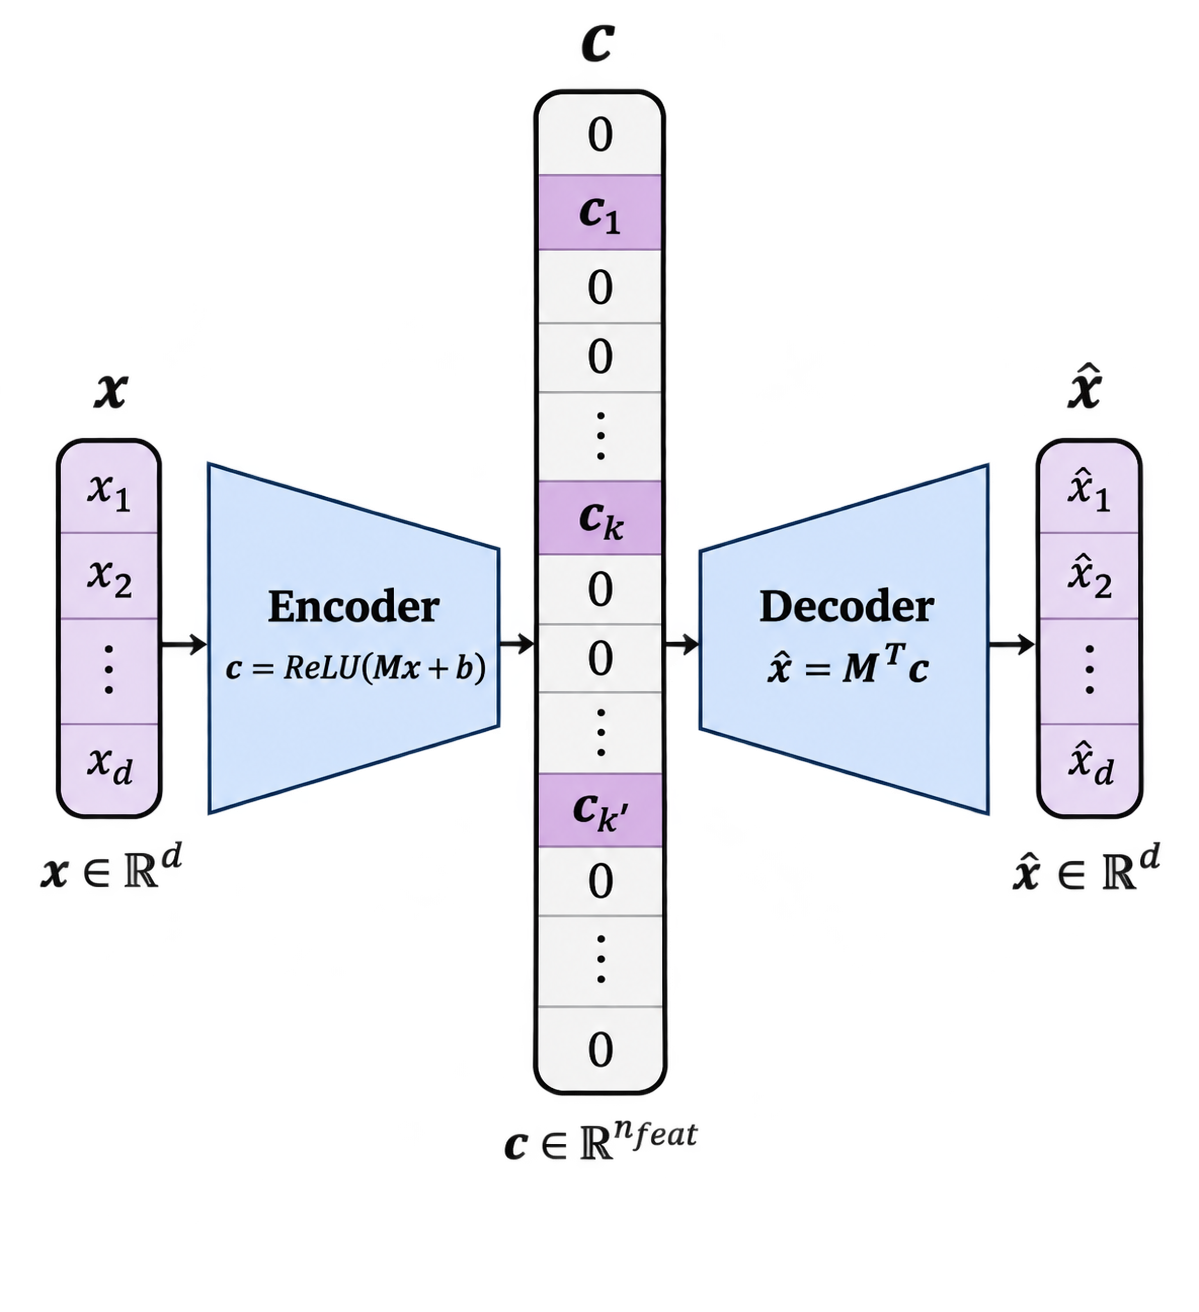
\includegraphics[width=\linewidth]{SAE.png}
    \end{column}
  \end{columns}
\end{frame}


\begin{frame}{Evaluating the Learned Features}

  The learned dictionary features are evaluated
  through two complementary experiments:

  \medskip

  \begin{itemize}

    \item \textbf{Experiment 1: Interpretability}

    Evaluates whether SAE features capture meaningful,
    interpretable concepts compared to alternative
    representations.

    \medskip

    \item \textbf{Experiment 2: Causal Evaluation}

    Investigates whether these features identify
    components causally responsible for specific
    model behaviors.

  \end{itemize}

\end{frame}


\section{Interpreting Dictionary Features}

\begin{frame}{Interpretability Evaluation}
  \small
  The first experiment evaluates whether the learned SAE features
  are less polysemantic and more interpretable than the original
  model representations.

  \medskip

  Interpretability is measured through an automated LLM-based evaluation:

  \begin{itemize}
    \item Collect text samples in which a dictionary feature activates.
    \item Use an LLM to generate a description of the feature from these samples.
    \item Use the description to predict the feature's activation on new text samples.
  \end{itemize}

  \medskip

  The \textbf{correlation} between predicted and actual activations
  defines the feature's \textbf{interpretability score}.

  \medskip

  \begin{table}
    \centering
    \footnotesize
    \setlength{\tabcolsep}{3pt}
    \begin{tabular}{c p{6.2cm} c}
      \hline
      \textbf{Feature} & \textbf{Description (GPT-4)} & \textbf{Score} \\
      \hline
      1-0000 & Parts of individual names, especially last names. & 0.33 \\
      1-0001 & Actions performed by a subject or object. & -0.11 \\
      1-0002 & Instances of 'W' and words beginning with 'w'. & 0.55 \\
      \hline
    \end{tabular}
  \end{table}
\end{frame}

\begin{frame}{Interpretability Results}
  \begin{columns}[c,onlytextwidth]
    \begin{column}{0.54\textwidth}
      \small
      SAE features are compared with the standard basis, random
      directions, PCA, and ICA in terms of interpretability.

      \medskip

      \begin{itemize}
        \item Sparse dictionary features achieve higher
        \textbf{interpretability scores}, especially in earlier layers.

        \item This advantage decreases in deeper layers, becoming
        comparable to ICA in layer 4 and minimal in the final layer.

        \item One possible explanation is that deeper features
        are more complex and harder for LLMs to interpret automatically.
      \end{itemize}
    \end{column}

    \begin{column}{0.44\textwidth}
      \centering
      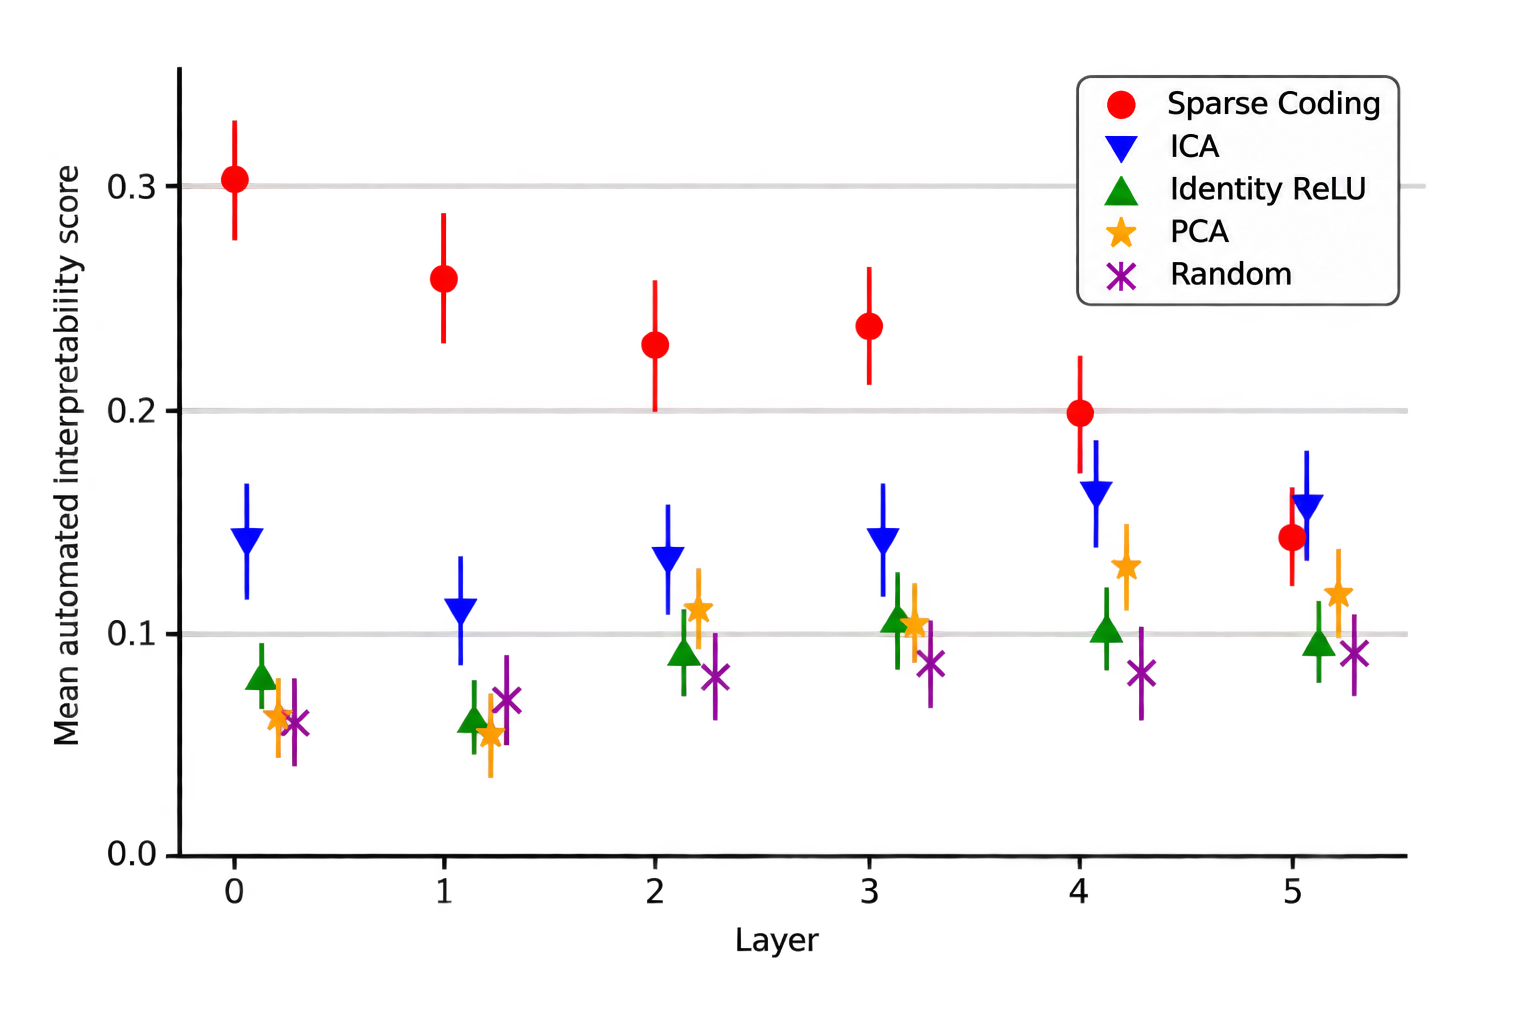
\includegraphics[width=\linewidth]{interpretability.png}
    \end{column}
  \end{columns}
\end{frame}

\section{Causal Evaluation}

\begin{frame}{Evaluating Causal Effects}
  \begin{columns}[c,onlytextwidth]
    \begin{column}{0.58\textwidth}
      \footnotesize
      The second experiment investigates whether learned dictionary
      features can identify components causally responsible for
      specific model behaviors.

      \medskip

      The evaluation focuses on the \textbf{Indirect Object
      Identification (IOI)} task, in which the model must predict
      the indirect object of a sentence.

      \medskip

      Through \textbf{activation patching}, selected feature contributions
      from a base sentence are replaced with those from a counterfactual
      target sentence.

      Features are ranked by causal importance and
      \textbf{progressively patched}.

      \medskip

      The effect is measured using \textbf{KL divergence} between the
      patched and target output distributions. Lower values indicate
      a closer match to the target predictions.
    \end{column}

    \begin{column}{0.40\textwidth}
      \centering
      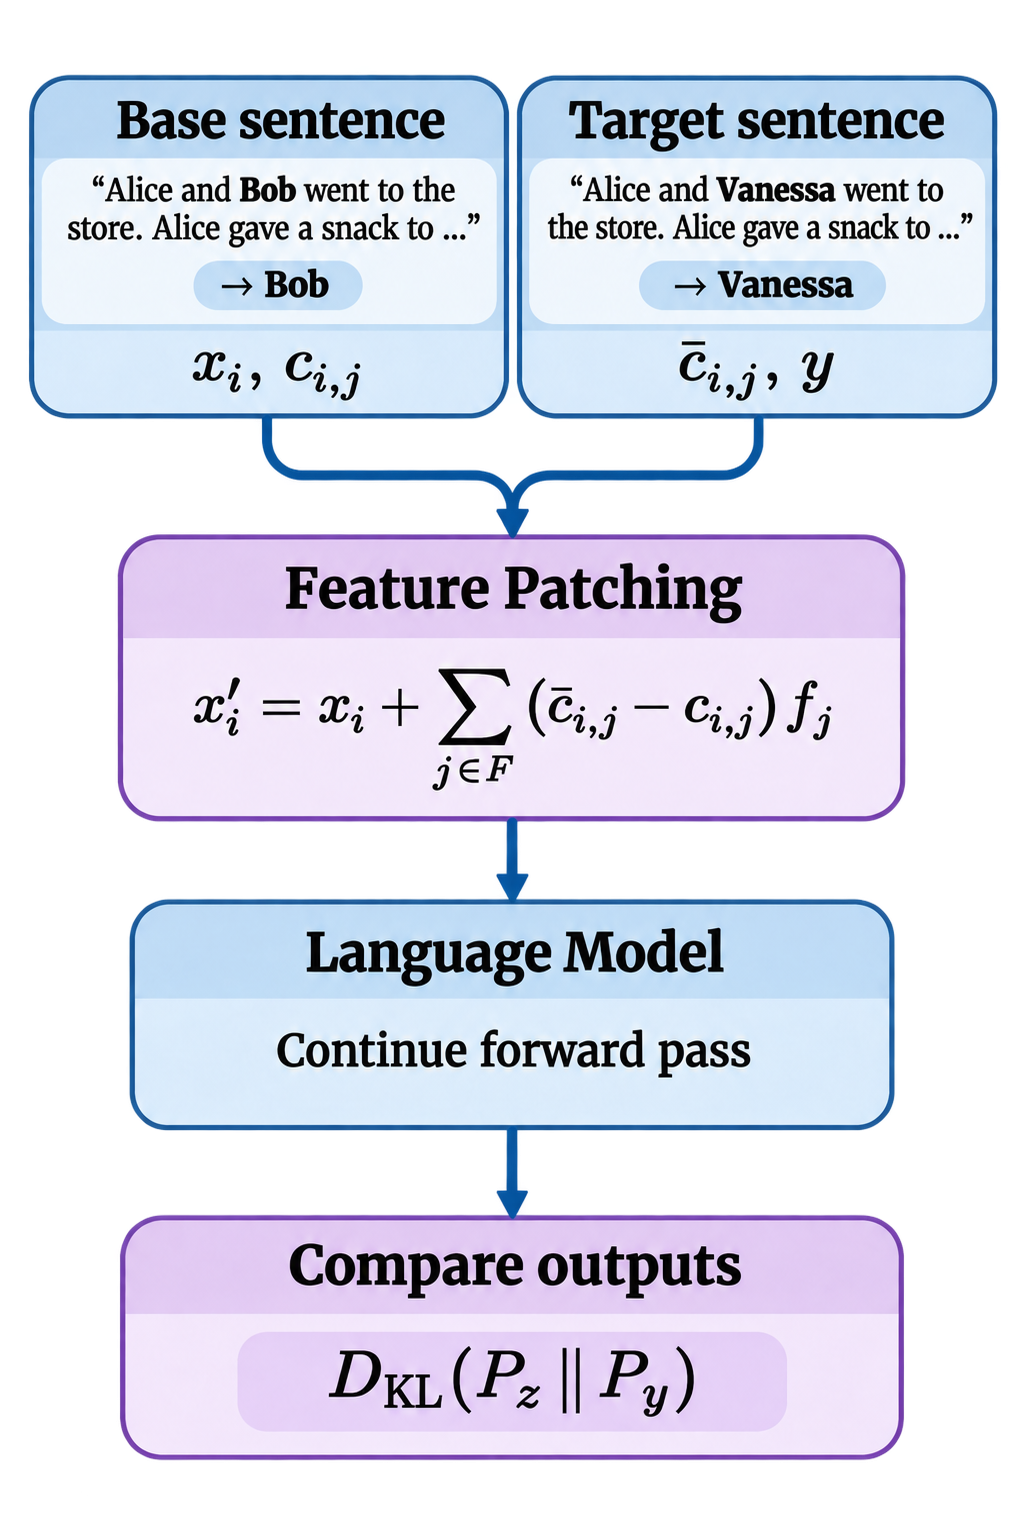
\includegraphics[
        width=\linewidth,
        height=0.85\textheight,
        keepaspectratio
      ]{causal.png}
    \end{column}
  \end{columns}
\end{frame}

\begin{frame}[t]{Causal Evaluation Results}
  \begin{minipage}[c][0.48\textheight][c]{\textwidth}
    \centering
    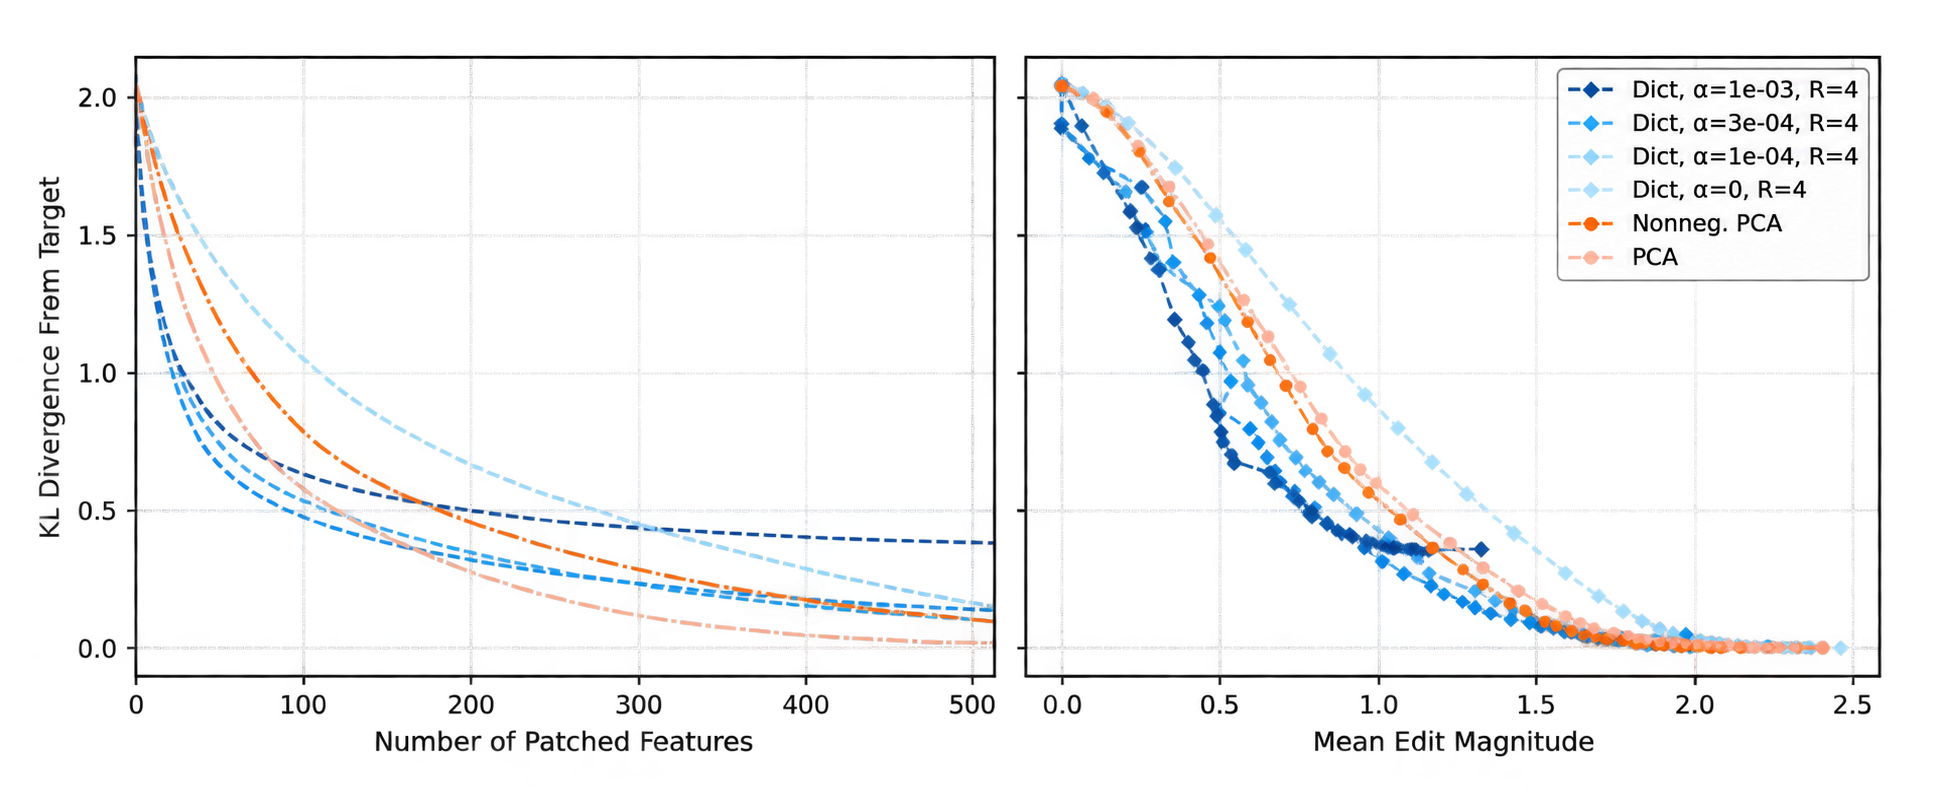
\includegraphics[
      width=0.95\linewidth,
      height=0.55\textheight,
      keepaspectratio
    ]{causalGraph.png}
  \end{minipage}

  \medskip
  \small
  Sparse dictionary features are compared with PCA and non-sparse dictionaries.

  \begin{itemize}
    \item Sparse dictionaries achieve the same KL divergence with
    \textbf{fewer patched features}.

    \item A better trade-off is achieved between \textbf{edit magnitude}
    and closeness to the target distribution.

    \item Increasing sparsity can reduce reconstruction accuracy,
    resulting in a higher minimum KL divergence.
  \end{itemize}
\end{frame}

\section{Case Studies}

\begin{frame}{Understanding Individual Features}
  Three complementary analyses examine the semantic meaning and
  causal role of dictionary features:

  \begin{itemize}
    \item \textbf{Input:} Identify the tokens and contexts associated
    with a feature's activation.

    \item \textbf{Output:} Measure how ablating the feature changes
    the model's output logits.

    \item \textbf{Intermediate features:} Identify features in earlier
    layers that contribute to the activation of the feature under study.
  \end{itemize}
\end{frame}

\begin{frame}[t]{Case Study 1: Monosemantic Features}
  \begin{minipage}[c][0.48\textheight][c]{\textwidth}
    \centering
    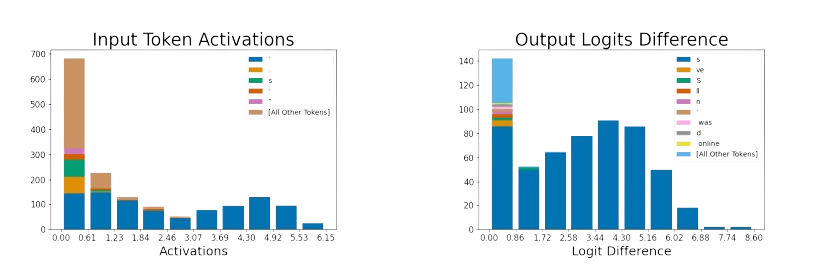
\includegraphics[
      width=0.95\linewidth,
      height=0.55\textheight,
      keepaspectratio
    ]{casestudy1.png}
  \end{minipage}

  \medskip
  \footnotesize
  A dictionary feature is analyzed through its input activations
  and the effect of ablation on the model's predictions.

  \begin{itemize}
    \item \textbf{Input activations:} The feature activates primarily
    on apostrophes, especially at higher activation values.

    \item \textbf{Output effect:} Ablating the feature mainly reduces
    the logit of the token ``s'', consistent with possessives and contractions.

    \item \textbf{Interpretation:} The feature exhibits a largely
    monosemantic pattern and a predictable causal effect on the output.
  \end{itemize}
\end{frame}

\begin{frame}{Case Study 2: Causal Circuits}
  \centering
  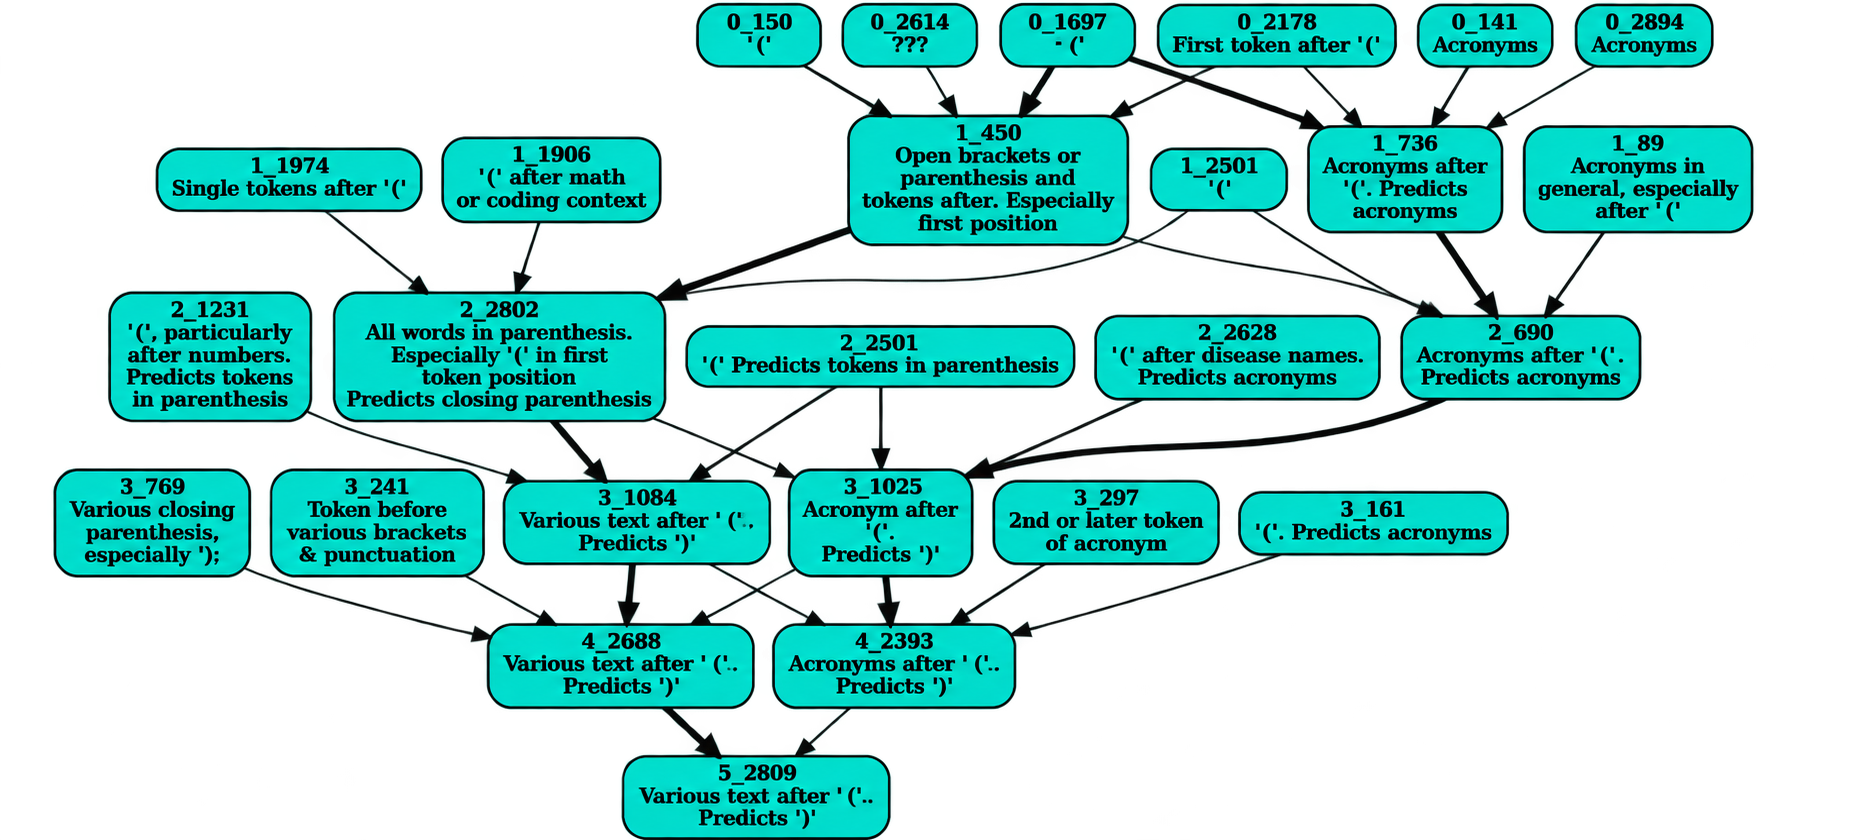
\includegraphics[
    width=0.95\linewidth,
    height=0.49\textheight,
    keepaspectratio
  ]{casestudy2.png}

  \vspace{0.5em}

  \begin{minipage}{0.95\textwidth}
    \small
    Interactions between dictionary features across layers are examined
    to identify interpretable causal circuits.

    Starting from a feature associated with predicting closing parentheses,
    contributions from earlier-layer features are traced.

    Selective ablations reveal a \textbf{causal tree} showing how
    different linguistic patterns contribute to the final prediction.
  \end{minipage}
\end{frame}


\begin{frame}{Limitations and Conclusions}

  \textbf{Limitations}

  \begin{itemize}
    \item Sparse dictionaries do not perfectly reconstruct
    the original activations, resulting in information loss.

    \item The method is mainly effective on residual streams,
    and causal results have only been demonstrated
    on the IOI task.
  \end{itemize}

  \bigskip

  \textbf{Conclusions}

  \begin{itemize}
    \item Sparse autoencoders learn more interpretable
    and often monosemantic features than traditional
    decomposition methods.

    \item These features allow more precise identification
    of causal components and support the discovery
    of interpretable circuits.
  \end{itemize}

\end{frame}
